
\documentclass[]{article}
\voffset=-1.5cm
\oddsidemargin=0.0cm
\textwidth = 480pt

% http://www.strath.ac.uk/aer/materials/5furtherquantitativeresearchdesignandanalysis/unit6/whatislogisticregression/

% http://www.medcalc.org/manual/logistic_regression.php


\usepackage{amsmath}
\usepackage{graphicx}
\usepackage{amssymb}
\usepackage{framed}
\usepackage{multicol}
%\usepackage[paperwidth=21cm, paperheight=29.8cm]{geometry}
%\usepackage[angle=0,scale=1,color=black,hshift=-0.4cm,vshift=15cm]{background}
%\usepackage{multirow}
\usepackage{enumerate}






\begin{document}
\subsection{One-way ANOVA in SPSS Statistics}

Introduction
The one-way analysis of variance (ANOVA) is used to determine whether there are any statistically significant differences between the means of two or more independent (unrelated) groups (although you tend to only see it used when there are a minimum of three, rather than two groups). For example, you could use a one-way ANOVA to understand whether exam performance differed based on test anxiety levels amongst students, dividing students into three independent groups (e.g., low, medium and high-stressed students). Also, it is important to realize that the one-way ANOVA is an omnibus test statistic and cannot tell you which specific groups were statistically significantly different from each other; it only tells you that at least two groups were different. Since you may have three, four, five or more groups in your study design, determining which of these groups differ from each other is important. You can do this using a post hoc test (N.B., we discuss post hoc tests later in this guide).

Note: If your study design not only involves one dependent variable and one independent variable, but also a third variable (known as a "covariate") that you want to "statistically control", you may need to perform an ANCOVA (analysis of covariance), which can be thought of as an extension of the one-way ANOVA. To learn more, see our SPSS Statistics guide on ANCOVA. Alternatively, if your dependent variable is the time until an event happens, you might need to run a Kaplan-Meier analysis.

This "quick start" guide shows you how to carry out a one-way ANOVA using SPSS Statistics, as well as interpret and report the results from this test. Since the one-way ANOVA is often followed up with a post hoc test, we also show you how to carry out a post hoc test using SPSS Statistics. However, before we introduce you to this procedure, you need to understand the different assumptions that your data must meet in order for a one-way ANOVA to give you a valid result. We discuss these assumptions next.

%====================================================%
Assumptions
When you choose to analyse your data using a one-way ANOVA, part of the process involves checking to make sure that the data you want to analyse can actually be analysed using a one-way ANOVA. You need to do this because it is only appropriate to use a one-way ANOVA if your data "passes" six assumptions that are required for a one-way ANOVA to give you a valid result. In practice, checking for these six assumptions just adds a little bit more time to your analysis, requiring you to click a few more buttons in SPSS Statistics when performing your analysis, as well as think a little bit more about your data, but it is not a difficult task.

Before we introduce you to these six assumptions, do not be surprised if, when analysing your own data using SPSS Statistics, one or more of these assumptions is violated (i.e., is not met). This is not uncommon when working with real-world data rather than textbook examples, which often only show you how to carry out a one-way ANOVA when everything goes well! However, don’t worry. Even when your data fails certain assumptions, there is often a solution to overcome this. First, let’s take a look at these six assumptions:

\begin{description}
\item[Assumption 1:] Your dependent variable should be measured at the interval or ratio level (i.e., they are continuous). Examples of variables that meet this criterion include revision time (measured in hours), intelligence (measured using IQ score), exam performance (measured from 0 to 100), weight (measured in kg), and so forth. You can learn more about interval and ratio variables in our article: Types of Variable.
\item[Assumption 2:] Your independent variable should consist of two or more categorical, independent groups. Typically, a one-way ANOVA is used when you have three or more categorical, independent groups, but it can be used for just two groups (but an independent-samples t-test is more commonly used for two groups). Example independent variables that meet this criterion include ethnicity (e.g., 3 groups: Caucasian, African American and Hispanic), physical activity level (e.g., 4 groups: sedentary, low, moderate and high), profession (e.g., 5 groups: surgeon, doctor, nurse, dentist, therapist), and so forth.
\item[Assumption 3:] You should have independence of observations, which means that there is no relationship between the observations in each group or between the groups themselves. For example, there must be different participants in each group with no participant being in more than one group. This is more of a study design issue than something you can test for, but it is an important assumption of the one-way ANOVA. If your study fails this assumption, you will need to use another statistical test instead of the one-way ANOVA (e.g., a repeated measures design). If you are unsure whether your study meets this assumption, you can use our Statistical Test Selector, which is part of our enhanced guides.
\item[Assumption 4:] There should be no significant outliers. Outliers are simply single data points within your data that do not follow the usual pattern (e.g., in a study of 100 students' IQ scores, where the mean score was 108 with only a small variation between students, one student had a score of 156, which is very unusual, and may even put her in the top 1\% of IQ scores globally). The problem with outliers is that they can have a negative effect on the one-way ANOVA, reducing the validity of your results. Fortunately, when using SPSS Statistics to run a one-way ANOVA on your data, you can easily detect possible outliers. In our enhanced one-way ANOVA guide, we: (a) show you how to detect outliers using SPSS Statistics; and (b) discuss some of the options you have in order to deal with outliers. You can learn more about our enhanced one-way ANOVA guide here.
\item[Assumption 5:] Your dependent variable should be approximately normally distributed for each category of the independent variable. We talk about the one-way ANOVA only requiring approximately normal data because it is quite "robust" to violations of normality, meaning that assumption can be a little violated and still provide valid results. You can test for normality using the Shapiro-Wilk test of normality, which is easily tested for using SPSS Statistics. In addition to showing you how to do this in our enhanced one-way ANOVA guide, we also explain what you can do if your data fails this assumption (i.e., if it fails it more than a little bit). Again, you can learn more here.
\item[Assumption 6:] There needs to be homogeneity of variances. You can test this assumption in SPSS Statistics using Levene's test for homogeneity of variances. If your data fails this assumption, you will need to not only carry out a Welch ANOVA instead of a one-way ANOVA, which you can do using SPSS Statistics, but also use a different post hoc test. In our enhanced one-way ANOVA guide, we (a) show you how to perform Levene’s test for homogeneity of variances in SPSS Statistics, (b) explain some of the things you will need to consider when interpreting your data, and (c) present possible ways to continue with your analysis if your data fails to meet this assumption, including running a Welch ANOVA in SPSS Statistics instead of a one-way ANOVA, and a Games-Howell test instead of a Tukey post hoc test (learn more here).
\end{description}
You can check assumptions 4, 5 and 6 using SPSS Statistics. Before doing this, you should make sure that your data meets assumptions 1, 2 and 3, although you don't need SPSS Statistics to do this. Remember that if you do not run the statistical tests on these assumptions correctly, the results you get when running a one-way ANOVA might not be valid. This is why we dedicate a number of sections of our enhanced one-way ANOVA guide to help you get this right. You can find out about our enhanced one-way ANOVA guide here, or more generally, our enhanced content as a whole here.

In the section, Test Procedure in SPSS Statistics, we illustrate the SPSS Statistics procedure to perform a one-way ANOVA assuming that no assumptions have been violated. First, we set out the example we use to explain the one-way ANOVA procedure in SPSS Statistics.

%=============================================================%
Example
A manager wants to raise the productivity at his company by increasing the speed at which his employees can use a particular spreadsheet program. As he does not have the skills in-house, he employs an external agency which provides training in this spreadsheet program. They offer 3 courses: a beginner, intermediate and advanced course. He is unsure which course is needed for the type of work they do at his company, so he sends 10 employees on the beginner course, 10 on the intermediate and 10 on the advanced course. When they all return from the training, he gives them a problem to solve using the spreadsheet program, and times how long it takes them to complete the problem. He then compares the three courses (beginner, intermediate, advanced) to see if there are any differences in the average time it took to complete the problem.

%==========================================%
\subsection{Setup in SPSS Statistics}
In SPSS Statistics, we separated the groups for analysis by creating a grouping variable called Course (i.e., the independent variable), and gave the beginners course a value of "1", the intermediate course a value of "2" and the advanced course a value of "3". Time to complete the set problem was entered under the variable name Time (i.e., the dependent variable). In our enhanced one-way ANOVA guide, we show you how to correctly enter data in SPSS Statistics to run a one-way ANOVA (see here). You can learn about our enhanced data setup content in general here. Alternately, we have a generic, "quick start" guide to show you how to enter data into SPSS Statistics, available here.

%==========================================%
\subsection{Test Procedure in SPSS Statistics}
The eight steps below show you how to analyse your data using a one-way ANOVA in SPSS Statistics when the six assumptions in the previous section, Assumptions, have not been violated. At the end of these eight steps, we show you how to interpret the results from this test. If you are looking for help to make sure your data meets assumptions 4, 5 and 6, which are required when using a one-way ANOVA, and can be tested using SPSS Statistics, you can learn more here.

\begin{itemize}
\item Step 1 Click Analyze > Compare Means > One-Way ANOVA... on the top menu, as shown below.
\end{itemize}
One-way ANOVA Menu
\begin{figure}
\centering
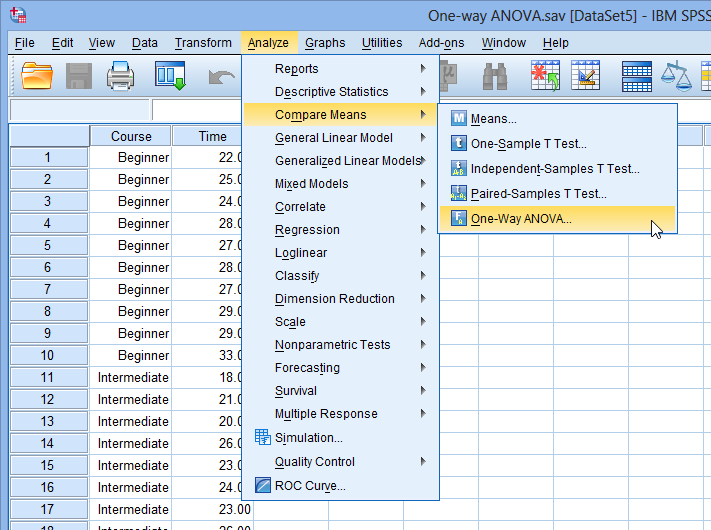
\includegraphics[width=0.7\linewidth]{images/one-way-anova-1}
\caption{}
\label{fig:one-way-anova-1}
\end{figure}

You will be presented with the One-Way ANOVA dialogue box:

One-way ANOVA Dialog Box
\begin{figure}[h!]
\centering
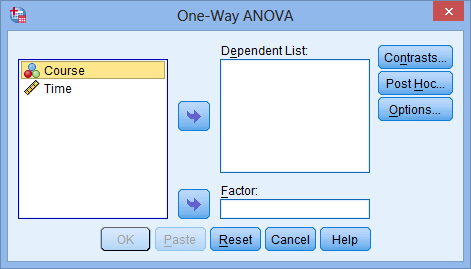
\includegraphics[width=0.7\linewidth]{images/one-way-anova-2}
\caption{}
\label{fig:one-way-anova-2}
\end{figure}
.
Transfer the dependent variable, Time, into the Dependent List: box and the independent variable, Course, into the Factor: box using the appropriate SPSS Right Arrow Button buttons (or drag-and-drop the variables into the boxes), as shown below:

One-way ANOVA Dialog Box
\begin{figure}[h!]
\centering
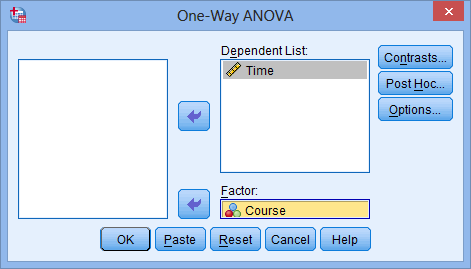
\includegraphics[width=0.7\linewidth]{images/one-way-anova-3}
\caption{}
\label{fig:one-way-anova-3}
\end{figure}

Click the SPSS Post Hoc Button button. Tick the Tukey checkbox as shown below:

One-way ANOVA  Post Hoc Dialog Box
\begin{figure}
\centering
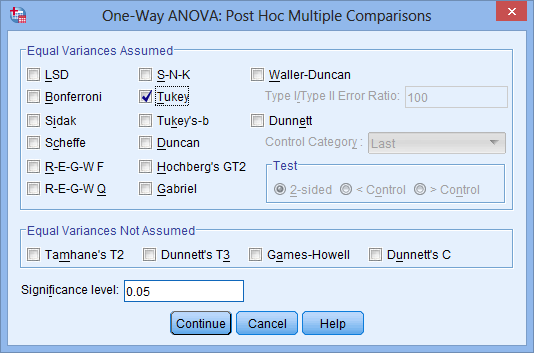
\includegraphics[width=0.7\linewidth]{images/one-way-anova-4}
\caption{}
\label{fig:one-way-anova-4}
\end{figure}

Click the  button.

%=============================================================%

One-way ANOVA Dialog Box
\begin{figure}
\centering
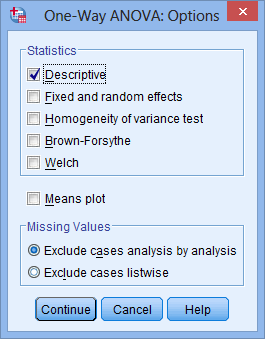
\includegraphics[width=0.7\linewidth]{images/one-way-anova-5}
\caption{}
\label{fig:one-way-anova-5}
\end{figure}

NOTE: When testing for some of the assumptions of the one-way ANOVA, you will need to tick more of these checkboxes. We take you through this, including how to interpret the output, in our enhanced one-way ANOVA guide.

Click the  button.

Click the  button.

%===========================================================================%
One-way ANOVA in SPSS Statistics (cont...)

SPSS Statistics Output of the one-way ANOVA
SPSS Statistics generates quite a few tables in its one-way ANOVA analysis. In this section, we show you only the main tables required to understand your results from the one-way ANOVA and Tukey post hoc test. For a complete explanation of the output you have to interpret when checking your data for the six assumptions required to carry out a one-way ANOVA, see our enhanced guide here. This includes relevant boxplots, and output from the Shapiro-Wilk test for normality and test for homogeneity of variances. Also, if your data failed the assumption of homogeneity of variances, we take you through the results for Welch ANOVA, which you will have to interpret rather than the standard one-way ANOVA in this guide. Below, we focus on the descriptives table, as well as the results for the one-way ANOVA and Tukey post hoc test only. We will go through each table in turn.

%===============================================================%
\subsection{Descriptives Table}
The descriptives table (see below) provides some very useful descriptive statistics, including the mean, standard deviation and 95\% confidence intervals for the dependent variable (Time) for each separate group (Beginners, Intermediate and Advanced), as well as when all groups are combined (Total). These figures are useful when you need to describe your data.

One-way ANOVA Output

\begin{figure}
\centering
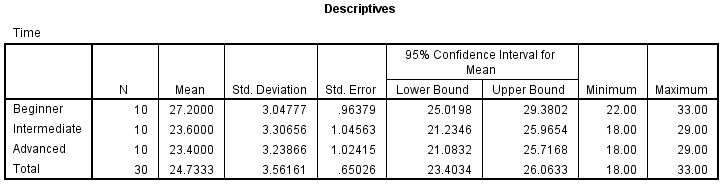
\includegraphics[width=0.7\linewidth]{images/one-way-anova-output-1}
\caption{}
\label{fig:one-way-anova-output-1}
\end{figure}

ANOVA Table
This is the table that shows the output of the ANOVA analysis and whether there is a statistically significant difference between our group means. We can see that the significance value is 0.021 (i.e., p = .021), which is below 0.05. and, therefore, there is a statistically significant difference in the mean length of time to complete the spreadsheet problem between the different courses taken. This is great to know, but we do not know which of the specific groups differed. Luckily, we can find this out in the Multiple Comparisons table which contains the results of the Tukey post hoc test.

One-way ANOVA Output
\begin{figure}[h!]
\centering
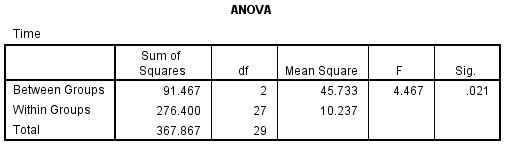
\includegraphics[width=0.7\linewidth]{images/one-way-anova-output-3}
\caption{}
\label{fig:one-way-anova-output-3}
\end{figure}

%============================================================%
\subsection{Multiple Comparisons Table}
From the results so far, we know that there are statistically significant differences between the groups as a whole. The table below, Multiple Comparisons, shows which groups differed from each other. The Tukey post hoc test is generally the preferred test for conducting post hoc tests on a one-way ANOVA, but there are many others. We can see from the table below that there is a statistically significant difference in time to complete the problem between the group that took the beginner course and the intermediate course (p = 0.046), as well as between the beginner course and advanced course (p = 0.034). However, there were no differences between the groups that took the intermediate and advanced course (p = 0.989).

One-way ANOVA Output
\begin{figure}
\centering
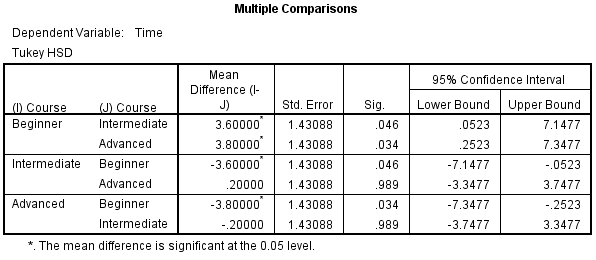
\includegraphics[width=0.7\linewidth]{images/one-way-anova-output-5}
\caption{}
\label{fig:one-way-anova-output-5}
\end{figure}
It is also possible to run comparisons between specific groups that you decided were of interest before you looked at your results. For example, you might have expressed an interest in knowing the difference in the completion time between the beginner and intermediate course groups. This type of comparison is often called a planned contrast or a simple custom contrast. However, you do not have to confine yourself to the comparison between two time points only. 

You might have had an interest in understanding the difference in completion time between the beginner course group and the average of the intermediate and advanced course groups. This is called a complex contrast. All these types of custom contrast are available in SPSS Statistics. 

In our enhanced guide we show you how to run custom contrasts in SPSS Statistics using syntax (or sometimes a combination of the graphical user interface and syntax) and how to interpret and report the results. In addition, we also show you how to "trick" SPSS Statistics into applying a Bonferroni adjustment for multiple comparisons which it would otherwise not do.

%===========================================================%
\subsection*{Reporting the output of the one-way ANOVA}
Based on the results above, you could report the results of the study as follows (N.B., this does not include the results from your assumptions tests or effect size calculations):

General
\begin{itemize}
	\item There was a statistically significant difference between groups as determined by one-way ANOVA (F(2,27) = 4.467, p = .021). A Tukey post hoc test revealed that the time to complete the problem was statistically significantly lower after taking the intermediate (23.6 ± 3.3 min, p = .046) and advanced (23.4 ± 3.2 min, p = .034) course compared to the beginners course (27.2 ± 3.0 min). There was no statistically significant difference between the intermediate and advanced groups (p = .989).
	
%\item In our enhanced one-way ANOVA guide, we show you how to write up the results from your assumptions tests, one-way ANOVA and Tukey post hoc results if you need to report this in a dissertation, thesis, assignment or research report. We do this using the Harvard and APA styles (see here). 
	
\item It is also worth noting that in addition to reporting the results from your assumptions, one-way ANOVA and Tukey post hoc test, you are increasingly expected to report an effect size. Whilst there are many different ways you can do this, we show you how to calculate an effect size from your SPSS Statistics results in our enhanced one-way ANOVA guide. 
\item Effect sizes are important because whilst the one-way ANOVA tells you whether differences between group means are "real" (i.e., different in the population), it does not tell you the "size" of the difference. Providing an effect size in your results helps to overcome this limitation. You can learn more about our enhanced one-way ANOVA guide here, or our enhanced content in general here.
\end{itemize}


\end{document}